\documentclass[10pt]{beamer}
\usetheme[
%%% option passed to the outer theme
%    progressstyle=fixedCircCnt,   % fixedCircCnt, movingCircCnt (moving is deault)
  ]{Feather}
  
% If you want to change the colors of the various elements in the theme, edit and uncomment the following lines

% Change the bar colors:
\setbeamercolor{Feather}{fg=red!80!black,bg=red!60!black}
\setbeamercolor{block title}{bg=red!80!black, fg=white}
\setbeamercolor{block body}{bg=white, fg=black}

% Change the color of the structural elements:
\setbeamercolor{structure}{fg=black}

% Change the frame title text color:
\setbeamercolor{frametitle}{fg=yellow}

% Change the normal text color background:
%\setbeamercolor{normal text}{fg=black,bg=gray!10}

%-------------------------------------------------------
% INCLUDE PACKAGES
%-------------------------------------------------------
\usepackage{ifpdf}
\usepackage{xcolor}
\usepackage{graphicx} 
\usepackage{caption}
\usepackage{subcaption}
\usepackage{multicol}
\usepackage{animate}
\usepackage{amsmath} 
\ifpdf
\DeclareGraphicsRule{*}{mps}{*}{}
\else
% Recent LaTeX versions donât require the next line
% \DeclareGraphicsRule{*}{eps}{*}{}
\fi

\usepackage[english, french]{babel}
\usepackage[utf8]{inputenc}
%\usepackage[TS1,T1]{fontenc}
%\usepackage{helvet}
\usepackage{fourier}
%\usepackage{hyperref}
%\usepackage{lmodern}
%\usepackage{mathrsfs}
\usepackage{natbib}
\usepackage{amsmath,amssymb,amsfonts,graphicx,shorttoc,textpos,caption,here, yfonts}
\usepackage{verbatim,enumerate,dsfont,fancyhdr,setspace,array}

%\usepackage[style=authoryear]{biblatex}
%\renewcommand*{\nameyeardelim}{\addcomma\addspace}


\graphicspath{{Feathergraphics/}}
%\bibliography{biblio1}
%\DeclareCiteCommand{\cite}
%{\usebibmacro{prenote}}
%{\usebibmacro{citeindex}%
%\usebibmacro{cite}}
%{\multicitedelim}
%{\usebibmacro{cite:postnote}}
%\usefonttheme[onlymath]{serif}
%\newbibmacro*{cite}{%
%\usebibmacro{cite:citepages}%
%\ifciteseen
%	{\iffieldundef{shorthand}
%		{\usebibmacro{cite:short}}
%		{\usebibmacro{cite:shorthand}}}
%	{\usebibmacro{cite:full}}}
%
%\renewbibmacro*{cite}{%
%\usebibmacro{cite:citepages}%
%{\usebibmacro{cite:full}}}
%-------------------------------------------------------
% DEFFINING AND REDEFINING COMMANDS
%-------------------------------------------------------

% colored hyperlinks
\newcommand{\chref}[2]{
  \href{#1}{{\usebeamercolor[bg]{Feather}#2}}
}
\DeclareMathOperator*{\argmin}{arg\,min}
%\bibliographystyle{apalike}
%\renewcommand\bibfont{\scriptsize}
\DeclareMathOperator*{\Argmin}{Arg\,min}
\setbeamertemplate{frametitle continuation}[from second]

%-------------------------------------------------------
% INFORMATION IN THE TITLE PAGE
%-------------------------------------------------------

\title[Optimal aggregation in circular deconvolution by a frequentist Bayesian approach] % [] is optional - is placed on the bottom of the sidebar on every slide
{ % is placed on the title page
\vspace*{8ex}
     \textbf{Optimal aggregation in circular deconvolution by a frequentist Bayesian approach}
}


\subtitle[loizeau@math.uni-heidelberg.de] % [] is optional - is placed on the bottom of the sidebar on every slide
{ % is placed on the title page
\vspace*{-2ex}
    StatMathAppli\\
    Fréjus
}


\institute[Ruprecht-Karls-Universität Heidelberg]
{
  \vspace*{8ex}
  \begin{flushright}Ruprecht-Karls-Universität Heidelberg\end{flushright}
  %there must be an empty line above this line - otherwise some unwanted space is added between the university and the country (I do not know why;( )
}

\date{\begin{flushleft}In collaboration with \\ Fabienne Comte and Jan Johannes\end{flushleft}}

\author[Xavier Loizeau] % [] is optional - is placed on the bottom of the sidebar on every slide
{ % is placed on the title page
\vspace*{-5ex}
      \textit{Xavier Loizeau\\      \hspace*{-6ex}$4^{th}$ of September 2017}
}
%-------------------------------------------------------
% THE BODY OF THE PRESENTATION
%-------------------------------------------------------

\begin{document}
%-------------------------------------------------------
% THE TITLEPAGE
%-------------------------------------------------------

{\1% % this is the name of the PDF file for the background
\begin{frame}[plain,noframenumbering] % the plain option removes the header from the title page, noframenumbering removes the numbering of this frame only
  \titlepage % call the title page information from above
\end{frame}}

\AtBeginSection[]{
\begin{frame}[noframenumbering]{Contents}
\setcounter{tocdepth}{1}
%\begin{multicols}{2}
\tableofcontents[sectionstyle=show/shaded, subsectionstyle=show/show/hide]
%\end{multicols}
\end{frame}
}

%\begin{frame}{Contents}
%\setcounter{tocdepth}{1}
%\tableofcontents
%\end{frame}

%-------------------------------------------------------
\section{Introduction}
%-------------------------------------------------------
\subsection{Considered model}

\begin{frame}{Considered model}{Circular deconvolution model}
\includegraphics<1>{deconv/pic.1}
\includegraphics<2>{deconv/pic.2}
\includegraphics<3>{deconv/pic.3}
\includegraphics<4>{deconv/pic.4}
\includegraphics<5>{deconv/pic.5}
\includegraphics<6>{deconv/pic.6}
\includegraphics<7->{deconv/pic.7}
\begin{itemize}
\item<3-> Object of interest: density of a circular r.v. $ X\sim f^{X}$;
\item<4-> Noise: circular r.v. $\epsilon \sim f^{\epsilon}$;
\item<5-> Observation: noisy circular r.v. $ Y=X+\epsilon \sim f^{Y} = f^{X} \star f^{\epsilon}$
\end{itemize}

\end{frame}


%\begin{frame}{Considered model}{Illustration}
%\begin{center}
%	\animategraphics[loop,controls,width=40ex]{10}{illu-deconv1/test-}{1}{25}
%\end{center}
%\end{frame}

\begin{frame}{Considered model}{Frequency domain}
As all our variables have values in $[0,1]$, their densities can be extended in Fourier series.
Hence we give the following definitions :

\medskip

\begin{itemize}
\setlength\itemsep{2em}
\item $\forall j \in \mathbb{Z}, x \in [0,1], \quad e_{j}(x) = \exp\left[- 2 \pi \cdot i \cdot j \cdot x\right]$, the Fourier basis;
\item $\left[f^{X}\right]_{j} = \mathbb{E}_{f^{X}}\left[e_{j}(-X_{1})\right]$, Fourier coefficients of $f^{X}$ ;
\item $\left[f^{\epsilon}\right]_{j} = \mathbb{E}_{f^{\epsilon}}\left[e_{j}(-\epsilon_{1})\right]$, the Fourier coefficients of $f^{\epsilon}$ ;
\item $\left[f^{Y}\right]_{j} = \mathbb{E}_{f^{Y}}\left[e_{j}(-Y_{1})\right] = \left[f^{X}\right]_{j} \cdot\left[f^{\epsilon}\right]_{j}$, the Fourier coefficients of $f^{Y}$;
\end{itemize}
\end{frame}

\begin{frame}{Considered model}{Illustration}
\begin{center}
	\animategraphics[loop,controls,width=40ex]{10}{illu-deconv2/}{800}{997}
\end{center}
\end{frame}

\subsection{Bayesian point of view}
\begin{frame}{Bayesian point of view}{Bayesian fondamental paradigm}
The problem is here treated from a Bayesian point of view:

\bigskip

\begin{itemize}
\setlength\itemsep{2em}
\item<1-> the parameter $\left[\boldsymbol{f}\right]$ is a random variable with \textcolor{red!90!black}{prior} $\textcolor{red!90!black}{\mathbb{P}_{\boldsymbol{\left[f\right]}}}$ with density $\pi_{\left[\boldsymbol{f}\right]}$ with respect to some measure;
\item<2-> given $\left[\boldsymbol{f}\right],$ the \textcolor{red!90!black}{likelihood} of $Y$ is $\textcolor{red!90!black}{\mathbb{P}_{Y \vert \left[\boldsymbol{f}\right]}^{n}}$ with density $\pi_{Y \vert \left[\boldsymbol{f}\right]}^{n}(y_{1}, \hdots, y_{n}, [f]) = \prod\limits_{k \in \llbracket 1, n \rrbracket}\sum\limits_{j \in \mathbb{Z}} \left[\boldsymbol{f}\right]_{j}\left[f^{\epsilon}\right]_{j} e_{j}(y_{k});$
\item<3-> the marginal distribution of $Y$ is $\mathbb{P}_{Y}^{n}$ ;
\item<4-> we are interested in the \textcolor{red!90!black}{posterior distribution} $\textcolor{red!90!black}{\mathbb{P}_{\left[\boldsymbol{f}\right] \vert Y}^{n}}$ with density $\pi_{\left[\boldsymbol{f}\right] \vert Y}^{n}([f], y)\propto \pi_{Y \vert \left[\boldsymbol{f}\right]}^{n}(y, [f]) \cdot \pi_{\left[\boldsymbol{f}\right]}([f]).$
\end{itemize}
\end{frame}

%\begin{frame}{Considered model}{Goal}
%\begin{itemize}
%	\item Frequentist point of view
%	\begin{itemize}
%		\item Define an estimator for the sequence $\left(\left[f^{X}\right]_{j}\right)_{j \in \mathbb{Z}}$, i.e. $\left(\widehat{\left[f\right]}_{j}\right)_{j \in \mathbb{Z}} : [0, 1]^{n} \rightarrow \mathcal{B}(0,1)^{\mathbb{Z}}$
%		\item Show that this estimator is "the best" for some criteria of interest
%	\end{itemize}
%	\item Bayesian point of view
%	\begin{itemize}
%		\item Define a prior distribution on $\mathcal{B}(0,1)^{\mathbb{Z}}$
%		\item Compute the posterior distribution
%		\item Study the behavior the random variables following this posterior distribution
%	\end{itemize}
%	\item Frequentist Bayesian point of view : show that the posterior is the best for some criterion
%\end{itemize}
%\end{frame}

\subsection{Frequentist case}
\begin{frame}{Formulation of optimality}{Frequentist case}
\begin{columns}
\begin{column}[T]{.4\textwidth}%
\hspace*{8ex}\includegraphics<1>[scale=.8]{./oraclefreq/inv-gssm.11}%
\includegraphics<2>[scale=.8]{./oraclefreq/inv-gssm.4}% lower
\includegraphics<3>[scale=.8]{./oraclefreq/inv-gssm.8}%
\includegraphics<4>[scale=.8]{./oraclefreq/inv-gssm.9}%
\includegraphics<5>[scale=.8]{./oraclefreq/inv-gssm.10}% upper + lower
\includegraphics<6>[scale=.8]{./oraclefreq/inv-gssm.5}%
\includegraphics<7>[scale=.8]{./oraclefreq/inv-gssm.6}%
\includegraphics<8->[scale=.8]{./oraclefreq/inv-gssm.7}%
\begin{textblock}{6}(2,14.5) \only<1->{Parameter of interest}\end{textblock} 
\end{column}\begin{column}[T]{.7\textwidth}%
\begin{itemize}
\item<2->
For each frequentist estimator, measure the performance by its risk
  \begin{equation*}
\mathbb{E}_{f^{X}}^{n} \left[d\left(\widetilde{f}, f^{X}\right)^{2}\right].
\end{equation*}
 \item<3->  Goal: \textcolor{red!90!black}{derive a lower bound} for this risk
\begin{equation*}
\inf\limits_{\widetilde{f}} \mathbb{E}_{f^{X}}^{n}\left[d\left(\widetilde{f}, f^{X}\right)^{2}\right] \geq \mathcal{R}_{n}^{\circ}\left(f^{X}\right)
\end{equation*}
over a family of estimators.
\item<6-> Finding $\widehat{f}$ in this family such that
  \begin{equation*}
\mathbb{E}_{f^{X}}^{n}\left[d\left(\widehat{f}, f^{X}\right)^{2}\right] \leq K^{\circ} \cdot \mathcal{R}_{n}^{\circ}\left(f^{X}\right),
\end{equation*}
it is then \textcolor{red!90!black}{oracle rate optimal} and \textcolor{red!90!black}{adaptive} if $\widehat{f}$ does not depend on $f^{X}$.
\end{itemize}
\end{column}
\end{columns}
\end{frame}

\subsection{Pragmatic Bayesian case}
\begin{frame}{Formulation of optimality}{Pragmatic Bayesian paradigm}
How to transfer this in a Bayesian point of view ?

\bigskip

Taking a "pragmatic Bayesian" point of view :

\bigskip

\begin{itemize}
\setlength\itemsep{3em}
\item $f^{X}$ the \textcolor{red!90!black}{true parameter}.
\item Is $\mathbb{P}_{\boldsymbol{f}\vert Y}^{n}$ \textcolor{red!90!black}{shrinking} around $f^{X}$ as $n$ tends to $\infty$ ?
\item How fast ?

\end{itemize}

\end{frame}


\begin{frame}{Formulation of optimality}{Pragmatic Bayesian formulation of optimality}
\begin{columns}
\begin{column}[T]{.4\textwidth}%
\hspace*{4ex}\includegraphics<1>[scale=.8]{./oraclebayes/reg.31}%
\includegraphics<2>[scale=.8]{./oraclebayes/reg.32}%
\includegraphics<3>[scale=.8]{./oraclebayes/reg.33}%
\includegraphics<4>[scale=.8]{./oraclebayes/reg.34}%
\includegraphics<5>[scale=.8]{./oraclebayes/reg.35}%
\includegraphics<6>[scale=.8]{./oraclebayes/reg.36}%
\includegraphics<7>[scale=.8]{./oraclebayes/reg.37}%
\includegraphics<8->[scale=.8]{./oraclebayes/reg.38}%
\end{column}\begin{column}[T]{.7\textwidth}%

\begin{itemize}

\item<1-> \textcolor{red!90!black}{Concentration rate} $(\phi_{n})_{n \in \mathbb{N}}$
\begin{alignat*}{2}
&\exists c \in \mathbb{R}_{+}, \quad \lim_{n \rightarrow \infty} \mathbb{E}_{f^{X}}^{n}&&\left[ \mathbb{P}_{\boldsymbol{f}\vert Y}^{n} \left(d\left(\boldsymbol{f}, f^{X} \right)^{2} \geq c \, \phi_{n} \right) \right] = 0.
\end{alignat*}

\item<5-> \textcolor{red!90!black}{Exact concentration rate} $(\phi_{n})_{n \in \mathbb{N}}$ if in addition

\[ \lim_{n \rightarrow \infty} \mathbb{E}_{f^{X}}^{n}\left[ \mathbb{P}_{\boldsymbol{f}\vert Y}^{n} \left(d\left(\boldsymbol{f}, f^{X} \right)^{2} \leq c^{-1} \, \phi_{n} \right) \right] = 0. \]

\end{itemize}
\end{column}
\end{columns}

\end{frame}

%\begin{frame}{Formulation of optimality}{Pragmatic Bayesian formulation of minimax optimality}
%\begin{itemize}
%\item Uniform concentration rate $(\phi_{n})_{n \in \mathbb{N}}$ over a subset on $\Theta^{\circ} \subset \Theta$
%\[  \lim_{n \rightarrow \infty} \sup_{f^{X} \in \Theta^{\circ}} \mathbb{E}_{f^{X}}^{n}\left[ \mathbb{P}_{\boldsymbol{f}\vert Y}^{n} \left(d\left( \boldsymbol{f}, f^{X} \right)^{2} \geq c \, \phi_{n} \right) \right] = 0.\]
%
%\item Exact uniform concentration rate $(\phi_{n})_{n \in \mathbb{N}}$ if in addition
%\[ \lim_{n \rightarrow \infty} \sup_{f^{X} \in \Theta^{\circ}} \mathbb{E}_{f^{X}}^{n}\left[ \mathbb{P}_{\boldsymbol{f}\vert Y}^{n} \left(d\left( \boldsymbol{f}, f^{X} \right)^{2} \leq c^{-1} \, \phi_{n} \right) \right] = 0. \]
%
%\end{itemize}
%\end{frame}



\subsection{A popular frequentist method}


\begin{frame}{A popular frequentist method}{Projection estimators}
From a frequentist point of view, a natural method to answer this problem is:

\bigskip

\begin{itemize}
\setlength\itemsep{2em}
\item<1-> define $\widehat{\left[f^{Y}\right]}_{j} = \frac{1}{n} \sum_{k = 1}^{n} e_{j}(-Y_{k})$, an unbiased estimator for $\left[f^{Y}\right]_{j} = \mathbb{E}_{f^{Y}}\left[e_{j}\left(-Y_{1}\right)\right]$ ;
\item<2-> consider $\widehat{\left[f\right]}_{j} = \frac{\widehat{\left[f^{Y}\right]}_{j}}{\left[f^{\epsilon}\right]_{j}}$, an unbiased estimator for $\left[f^{X}\right]_{j}$ ;
\item<3-> use an element from the family of projection estimators : $\left\{\left(\widehat{\left[f\right]}^{m}_{j}\right)_{j \in \mathbb{Z}} : \forall j \in \mathbb{Z}, \quad \widehat{\left[f\right]}^{m}_{j} = \widehat{\left[f\right]}_{j} \mathds{1}_{\left\{0 < \vert j \vert \leq m\right\}} + \mathds{1}_{\left\{j = 0\right\}} \right\};$
\item<4-> define a method to select $m$ in a satisfactory way (e.g. \citet{PM}).
\end{itemize}

\end{frame}

%\begin{frame}{A popular frequentist method}{Model selection}
%One would select $m$ in such a way that minimize the risk which is given by
%\begin{alignat*}{3}
%&\mathbb{E}_{f^{X}}\left[\left\Vert \widehat{\left[f\right]} - \left[f^{X}\right]\right\Vert^{2}\right] &&=&& \sum\limits_{0 < \vert j \vert \leq m} \mathbb{V}\left[\widehat{\left[f\right]} \right] + \sum\limits_{\vert j \vert > m} \left\vert \left[f^{X}\right]_{j}\right\vert ^{2}\\
%& && = && \sum\limits_{0 < \vert j \vert \leq m} \frac{1 - \left\vert \left[f^{Y}\right]_{j}\right\vert^{2}}{n \cdot \left\vert\left[f^{\epsilon}\right]_{j}\right\vert^{2} } + \sum\limits_{\vert j \vert > m} \left\vert \left[f^{X}\right]_{j}\right\vert ^{2}\\
%\end{alignat*}
%
%\underline{Idea :} minimizing a penalized contrast which estimate the risk
%\[-\left\Vert \widehat{\left[f\right]}^{m} \right\Vert^{2} + pen_{m}\]
%\end{frame}

\subsection{Illustration}
\begin{frame}{Illustration}{Direct case}
\begin{figure}
\centering
 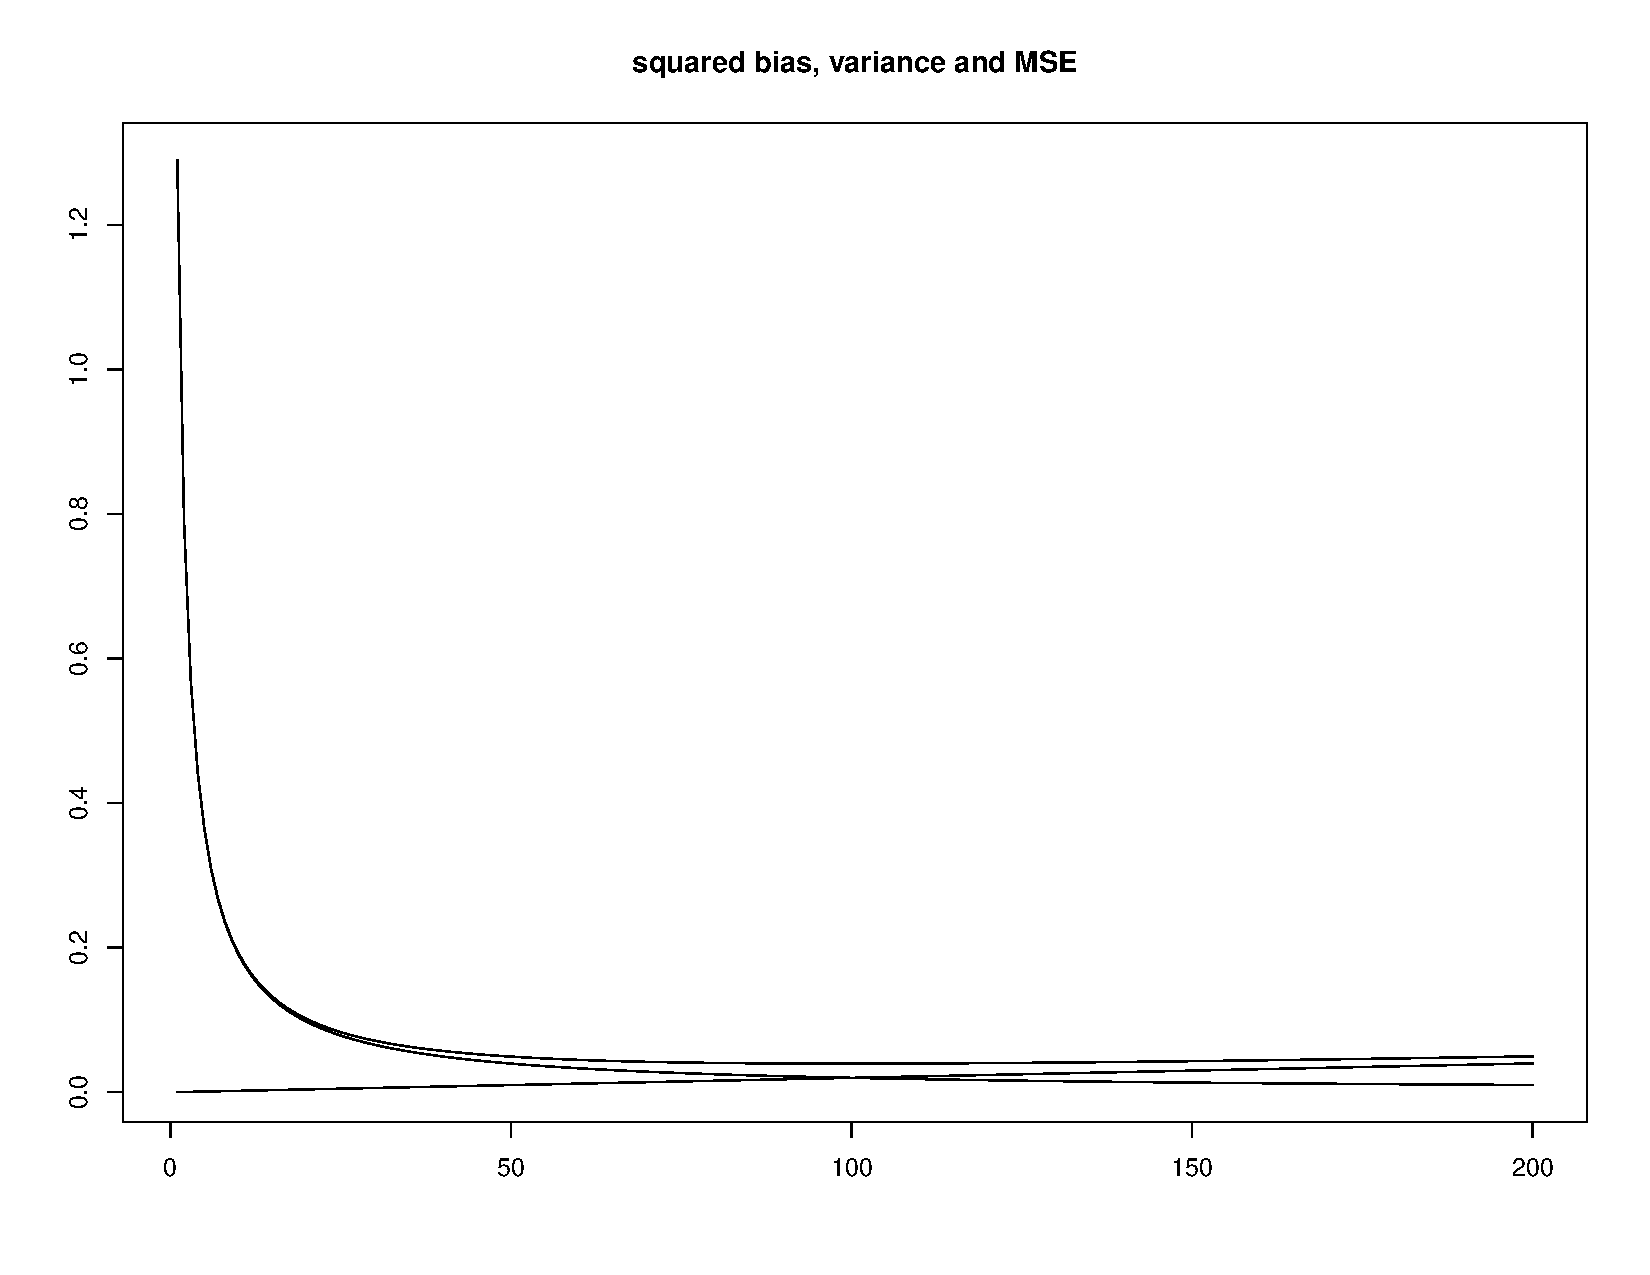
\includegraphics[width=.8\linewidth]{direct-case.pdf}
\caption{MSE of projection estimators in the direct case}\label{DC}
\end{figure}
\end{frame}

\begin{frame}{Illustration}{Direct case}
\begin{center}
	\animategraphics[loop,controls,width=40ex]{10}{anim-proj/}{1}{91}
\end{center}
\end{frame}

\begin{frame}{Illustration}{Inverse case}
\begin{figure}
\centering
 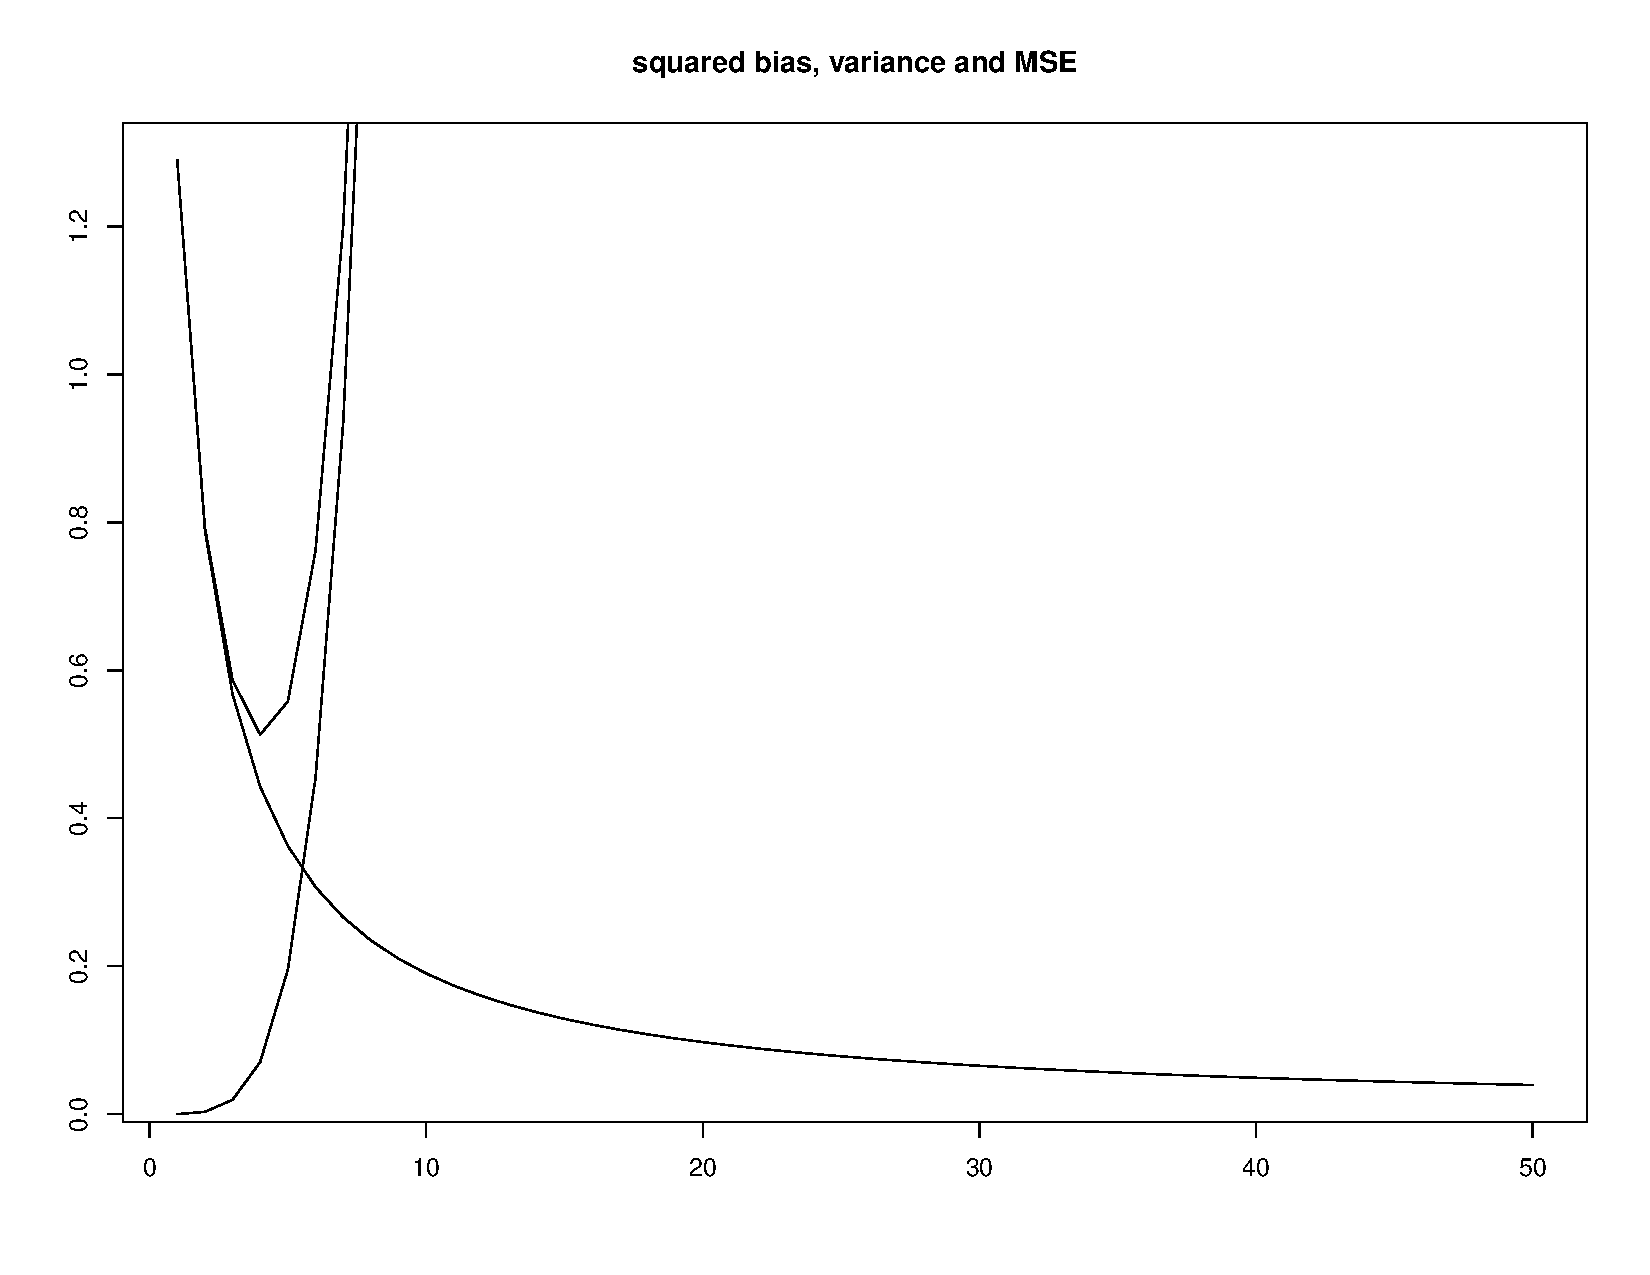
\includegraphics[width=.8\linewidth]{mildly-illposed.pdf}
\caption{MSE of projection estimators in the mildly ill-posed case case}\label{DC}
\end{figure}
\end{frame}

\begin{frame}{Considered model}{Illustration}
\begin{center}
	\animategraphics[loop,controls,width=40ex]{10}{anim-proj-expo/}{1}{34}
\end{center}
\end{frame}

\section{Suggested method}
\subsection{Sieve priors}

\begin{frame}{Sieve prior}{Prior form}
We first introduce the so called sieve priors with deterministic threshold parameter $m$ :
\begin{alignat*}{3}
&\pi_{\left[\boldsymbol{f}\right]}\left(\left[f\right]\right) &&=&& \prod\limits_{\left\vert j \right\vert > m} \delta_{0}\left(\left[f\right]_{j}\right)\cdot\exp\left[\Delta_{1}\left(\left[f\right]\right)\right].
\end{alignat*}

%This approach is motivated by the scheme applied to the Gaussian sequence space model in \citet{JJXL}.
\end{frame}

\begin{frame}{Sieve prior}{Posterior form}
The posterior is then of the form
\begin{alignat*}{2}
&\pi_{\left[\boldsymbol{f}\right] \vert Y^{n}}&&\left(\left[f\right], y^{n}\right) = \prod\limits_{\left\vert j \right\vert > m} \delta_{0}\left(\left[f\right]_{j}\right) \cdot\\
& && \exp\left[\underbrace{\Delta_{1}\left(\left[f\right]\right) + \sum\limits_{k = 1}^{n} \log\left(1 + \sum\limits_{0 < \vert j \vert \leq m} \left[f\right]_{j} \cdot \left[f^{\epsilon}\right]_{j} \cdot e_{j}(y_{k})\right) + \Delta_{2}(y^{n})}_{R\left(\left[f\right], y^{n}\right)}\right].
\end{alignat*}
\end{frame}

%\begin{frame}{Sieve prior}{Posterior approximated form}
%\underline{Open question :}
%By using a Taylor expansion of the $\log$ around $1$, it seems like this distribution could be approximated by a Gaussian, indeed
%\begin{alignat*}{4}
%& R\left(\left[f\right], y^{n}\right) &&=&& \Delta_{1}(\left[ f \right]) +&& \sum\limits_{k=1}^{n}\sum\limits_{l = 1}^{\infty} \frac{(-1)^{l+1}}{l} \left(\sum\limits_{0 < \vert j \vert \leq m} \left[ f \right]_{j} \cdot \left[ f^{\epsilon} \right]_{j} \cdot e_{j}(y_{k})\right)^{l} + \Delta_{2}(y^{n})\\
%& && = && \Delta_{1}(\left[ f \right]) +&& \sum\limits_{0 < \vert j \vert \leq m} \sum\limits_{k=1}^{n} \left[ f \right]_{j} \cdot \left[ f^{\epsilon} \right]_{j} \cdot e_{j}(y_{k}) + \Delta_{2}(y^{n})\\
%& && && &&+ \sum\limits_{l = 2}^{\infty}\sum\limits_{k=1}^{n} \frac{(-1)^{l+1}}{l} \left(\sum\limits_{0 < \vert j \vert \leq m} \left[ f \right]_{j} \cdot \left[ f^{\epsilon} \right]_{j} \cdot e_{j}(y_{k})\right)^{l}\\
%& && = && [...] &&
%\end{alignat*}
%\end{frame}

\begin{frame}{Sieve prior}{Posterior approximated form}
\underline{Open question :}
By using a Taylor expansion of the $\log$ around $1$, it seems like this distribution could be approximated by a Gaussian, indeed :
\begin{alignat*}{3}
& R\left(\left[f\right], y^{n}\right) &&=&& -\sum\limits_{0 < \vert j \vert \leq m}\frac{ \left\vert \left[ f \right]_{j} - \widehat{\left[ f \right]}_{j} \right\vert^{2}}{2 \cdot \sigma_{j}}\\
& && && + \sum\limits_{l = 2}^{\infty}\sum\limits_{k=1}^{n} \frac{(-1)^{l+1}}{l} \left(\sum\limits_{0 < \vert j \vert \leq m} \left[ f \right]_{j} \cdot \left[ f^{\epsilon} \right]_{j} \cdot e_{j}(y_{k})\right)^{l} + \delta_{1}\left(\left[f\right]\right) + \delta_{2}\left(y^{n}\right) ;
\end{alignat*}
where $\sigma_{j} = \frac{1}{1 + n \left\vert\left[f^{\epsilon}\right]_{j}\right\vert^{2}}$ and $\widehat{\left[f\right]}_{j} = \frac{\left[f^{\epsilon}\right]_{j} \cdot \sum\limits_{k = 1}^{n}e_{j}(y_{k})}{1 + n \left\vert\left[f^{\epsilon}\right]_{j}\right\vert^{2}}$
\end{frame}

\begin{frame}{Looking for a prior}{Hierarchical prior}
\begin{itemize}
\item Consider a \textcolor{red!90!black}{random hyper-parameter} \textcolor{red!90!black}{$M$}, with values in $\llbracket 1, n \rrbracket$, acting like a threshold:
\begin{align*}
\forall j \in \mathbb{Z} : \vert j \vert > m ,& \quad \mathbb{P}_{\left[\boldsymbol{f}\right]_{j}\vert M = m} = \delta_{0}
\end{align*}
\item Write the density of $M$ \textcolor{red!90!black}{$\pi_{M}(m) \propto \exp\left[pen(m)\right]$} with respect to the counting measure, then, the posterior can be written
\textcolor{red!90!black}{
\begin{alignat*}{2}
&\pi_{M \vert Y^{n}}(m, y^{n}) && = \exp\left[pen(m) - 2 \Delta_{2}(y^{n})\right]\\
%& && = \exp\left[-\sum\limits_{0 < \vert j\vert \leq m}\left\vert \left[ f^{\epsilon} \right]_{j} \cdot \sum\limits_{k = 1}^{n} e_{j}(y_{k}) \right\vert^{2} + pen(m)\right] \cdot \exp\left[\delta_{2}(y^{n}) + ...\right]\\
&\pi_{\left[\boldsymbol{f}\right]\vert Y^{n}} &&= \sum\limits_{m \in \mathbb{N}} \pi_{\left[\boldsymbol{f}\right] \vert M = m, Y^{n}} \cdot \pi_{M = m \vert Y^{n}};\\
&\widetilde{\left[\boldsymbol{f}\right]} &&= \left(\mathbb{E}_{\left[\boldsymbol{f}\right] \vert M \geq j, Y^{n}}\left[\left[\boldsymbol{f}\right]_{j}\right] \cdot \mathbb{P}_{M \vert Y^{n}}\left(M \geq j\right)\right)_{j \in \mathbb{N}}.
\end{alignat*}}
\end{itemize}

\end{frame}


\begin{frame}{Hierarchical prior}{Graphical representation}
\begin{center}
	\animategraphics[loop,controls,width=40ex]{10}{distM/}{1}{100}
\end{center}
\end{frame}

\section{Optimality results}
\begin{frame}{Optimality results}{Definitions}
We here note :
%\begin{itemize}
%\item $\Phi_{n}^{\circ} = \Phi_{n}^{\circ}\left(\left[f^{X}\right]\right)$ the optimal convergence rate for the family of projection estimators for each $\left[f^{X}\right]$;
%\item $\Phi_{n}^{\star} = \Phi_{n}^{\star}\left(\Theta^{\circ}\right)$ the minimax optimal convergence rate over some Sobolev ellipsoid $\Theta^{\circ}$.
%\end{itemize}
$\Phi_{n}^{\circ} = \Phi_{n}^{\circ}\left(\left[f^{X}\right]\right)$ the optimal convergence rate for the family of projection estimators for each $\left[f^{X}\right]$; this objects has analytical formulation (see for example \citet{FCMLT}).
\end{frame}


\subsection{Optimality of the Bayes estimate}
\begin{frame}{Optimality of the Bayes estimate}
\begin{block}<1->{Theorem : oracle optimality \textbf{J \& C \& L [2017]}}
For each $\left[f^{X}\right]$, there exist $C^{\circ}$ such that
	\[\forall n, \in \mathbb{N}^{\star}, \quad \mathbb{E}_{\left[f^{X}\right]}^{n}\left[\left\Vert \widetilde{\left[\boldsymbol{f}\right]} - \left[f^{X}\right] \right\Vert^{2}\right] \leq C^{\circ} \Phi_{n}^{\circ}.\]
\end{block}
%\begin{block}<2->{Theorem : minimax optimality \textbf{J \& C \& L [2017]}}
%There exist $C^{\star}$ such that
%	\[\forall n \in \mathbb{N}^{\star}, \quad \sup\limits_{\left[f^{X}\right]\in \Theta^{\circ}}\mathbb{E}_{\left[f^{X}\right]}^{n}\left[\left\Vert \widetilde{\left[\boldsymbol{f}\right]} - \left[f^{X}\right] \right\Vert^{2}\right] \leq C^{\star} \Phi_{n}^{\star}.\]
%\end{block}

\end{frame}

\subsection{Optimality of the posterior distribution}

\begin{frame}{Optimality of the posterior distribution}{Optimal contraction rates}

\begin{block}{Theorem J \& C \& L [2017]}
$\Phi_{n}^{\circ}$ can be considered as upper bound for the family of sieve priors :
%$\Phi_{n}^{\circ}$ and $\Phi_{n}^{\star}$ can be considered as upper bounds for the family of sieve priors :
%\begin{itemize}
%\item $\lim\limits_{n \rightarrow \infty} \inf\limits_{\mathbb{Q}_{\left[\boldsymbol{f}\right]}}\, \mathbb{E}_{\left[ f^{X} \right]}^{n}\left[\mathbb{Q}_{\left[\boldsymbol{f}\right] \vert Y^{n}}\left(\left\Vert \left[\boldsymbol{f}\right] - \left[ f^{X}\right] \right\Vert^{2} \geq \Phi_{n}^{\circ}\right)\right] = 1$,
%\item $\lim\limits_{n \rightarrow \infty} \inf\limits_{\mathbb{Q}_{\left[\boldsymbol{f}\right]}}\sup\limits_{\left[ f^{X} \right] \in \Theta^{\circ}}\, \mathbb{E}_{\left[f^{X}\right]}^{n}\left[\mathbb{Q}_{\left[\boldsymbol{f}\right] \vert Y^{n}}^{n}\left(\left\Vert \left[\boldsymbol{f}\right] - \left[ f^{X}\right] \right\Vert^{2} \geq \Phi_{n}^{\star}\right)\right] = 1$,
%\end{itemize}
\[\lim\limits_{n \rightarrow \infty} \inf\limits_{\mathbb{Q}_{\left[\boldsymbol{f}\right]}}\, \mathbb{E}_{\left[ f^{X} \right]}^{n}\left[\mathbb{Q}_{\left[\boldsymbol{f}\right] \vert Y^{n}}\left(\left\Vert \left[\boldsymbol{f}\right] - \left[ f^{X}\right] \right\Vert^{2} \geq \Phi_{n}^{\circ}\right)\right] = 1,\]
where $\inf_{\mathbb{Q}_{\left[\boldsymbol{f}\right]}}$ is taken over the family of sieve priors with Gaussian margins.
\end{block}
This gives a purely Bayesian formulation of oracle optimality.

% Could the second expression be a first step towards a purely Bayesian formulation of minimax optimality ?
\end{frame}

\begin{frame}{Optimality of the posterior distribution}
\begin{block}<1->{Theorem : oracle concentration \textbf{J \& C \& L [2017]}}
For all $\left[f^{X}\right]$ in $\Theta^{\circ}$, there exist $K^{\circ}$ such that
	\[\lim\limits_{n \rightarrow \infty} \mathbb{E}_{\left[f^{X}\right]}^{n}\left[\mathbb{P}_{\left[\boldsymbol{f}\right], M \vert Y^{n}}\left(\left(K^{\circ}\right)^{-1} \Phi_{n}^{\circ} \leq \left\Vert \left[\boldsymbol{f}\right] - \left[f^{X}\right] \right\Vert^{2} \leq K^{\circ} \Phi_{n}^{\circ} \right)\right] = 1.\]
\end{block}
%\begin{block}<2->{Theorem : minimax concentration \textbf{J \& C \& L [2017]}}
%For any unbounded sequence $K_{n}$, we have
%	\[\lim\limits_{n \rightarrow \infty} \sup\limits_{\left[f^{X}\right] \in \Theta^{\circ}} \mathbb{E}_{\left[f^{X}\right]}^{n}\left[\mathbb{P}_{\left[\boldsymbol{f}\right], M \vert Y^{n}}\left(\left\Vert \left[\boldsymbol{f}\right] - \left[f^{X}\right] \right\Vert^{2} \leq K_{n} \Phi_{n}^{\star} \right)\right] = 1.\]
%\end{block}
\end{frame}

\section{Simulations}
\begin{frame}{Direct case : visualisation of the estimates}
\begin{center}
	\animategraphics[loop,controls,width=40ex]{10}{compare-direct/}{1}{136}
\end{center}
\end{frame}

\begin{frame}{Direct case : sampling from the approximated posterior}
\begin{figure}
\centering
 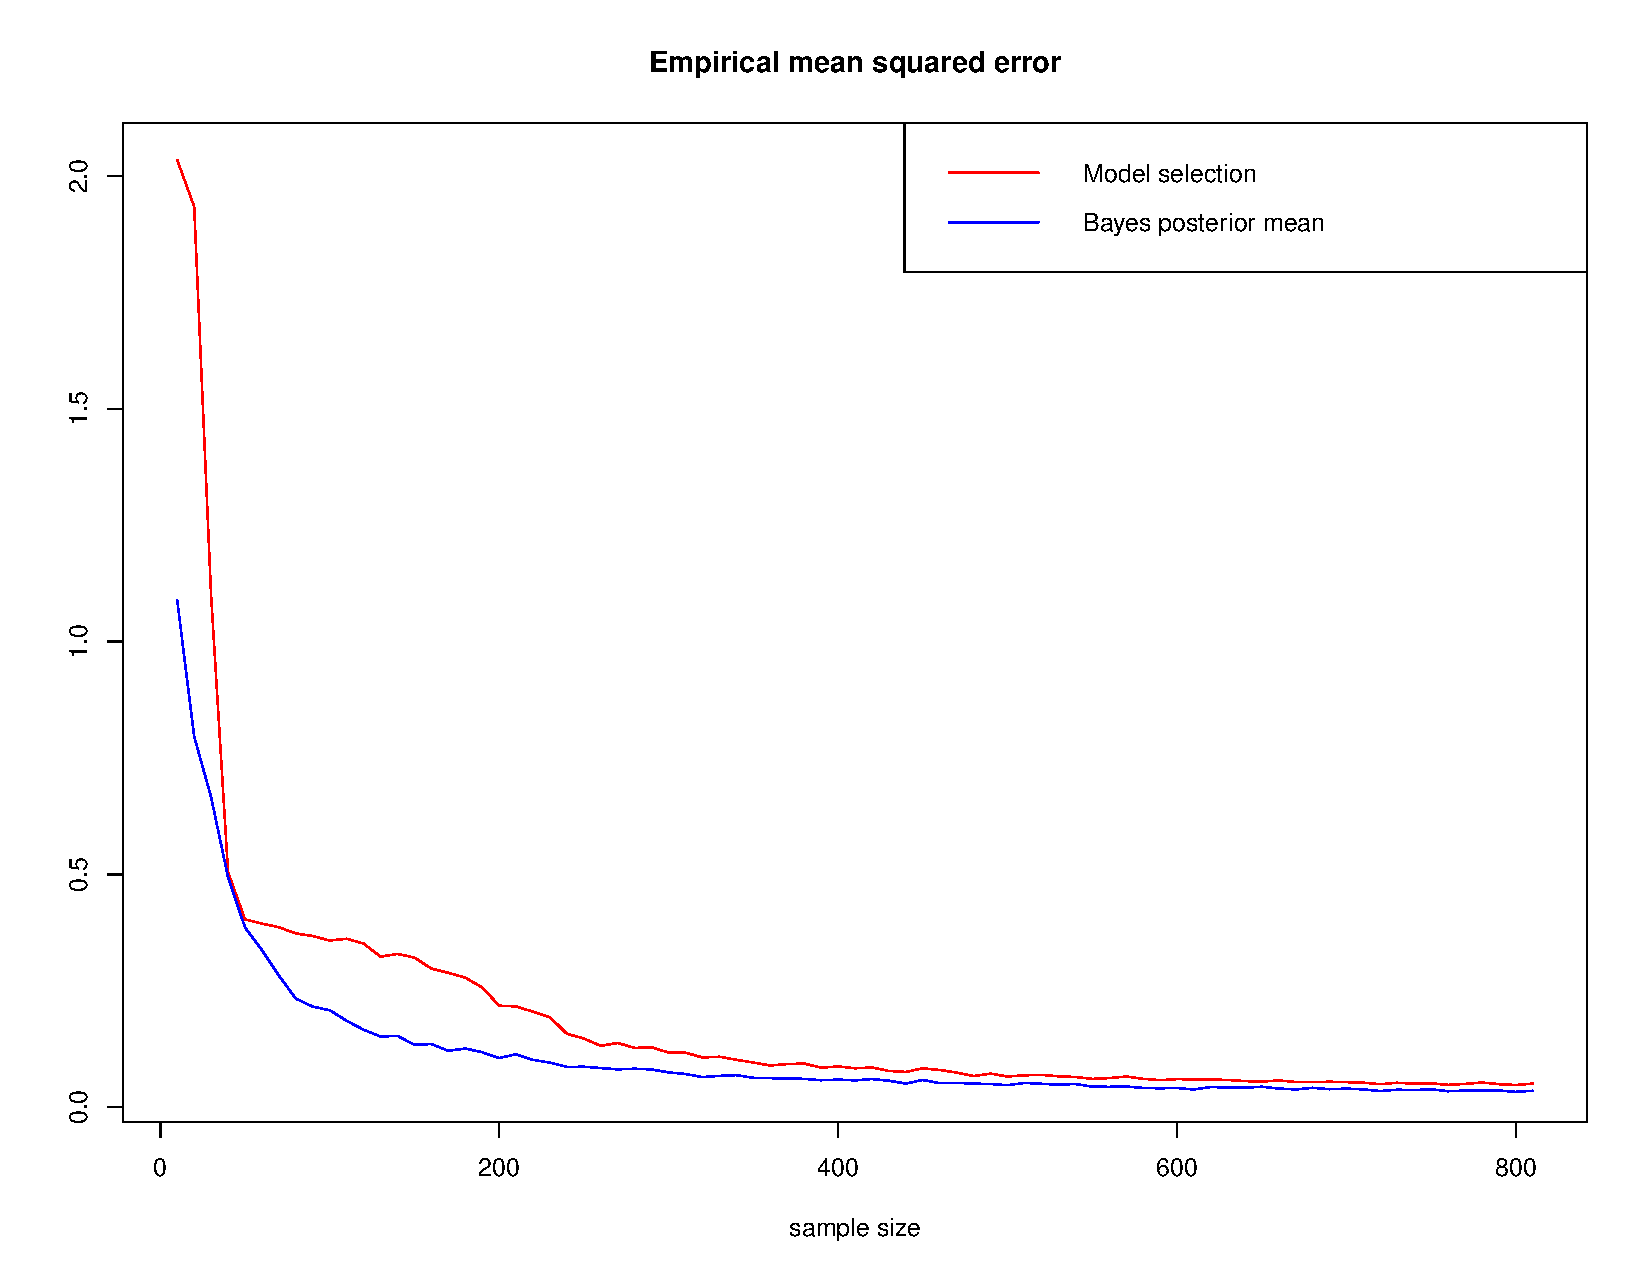
\includegraphics[width=.75\linewidth]{EQMdirect.pdf}
\caption{Evolution of the empirical mean squared error of the two estimates with respect to the number of observations in the direct case}\label{M}
\end{figure}
\end{frame}

\begin{frame}{Direct case : empirical mean square errors of the estimates}
\begin{figure}
\centering
 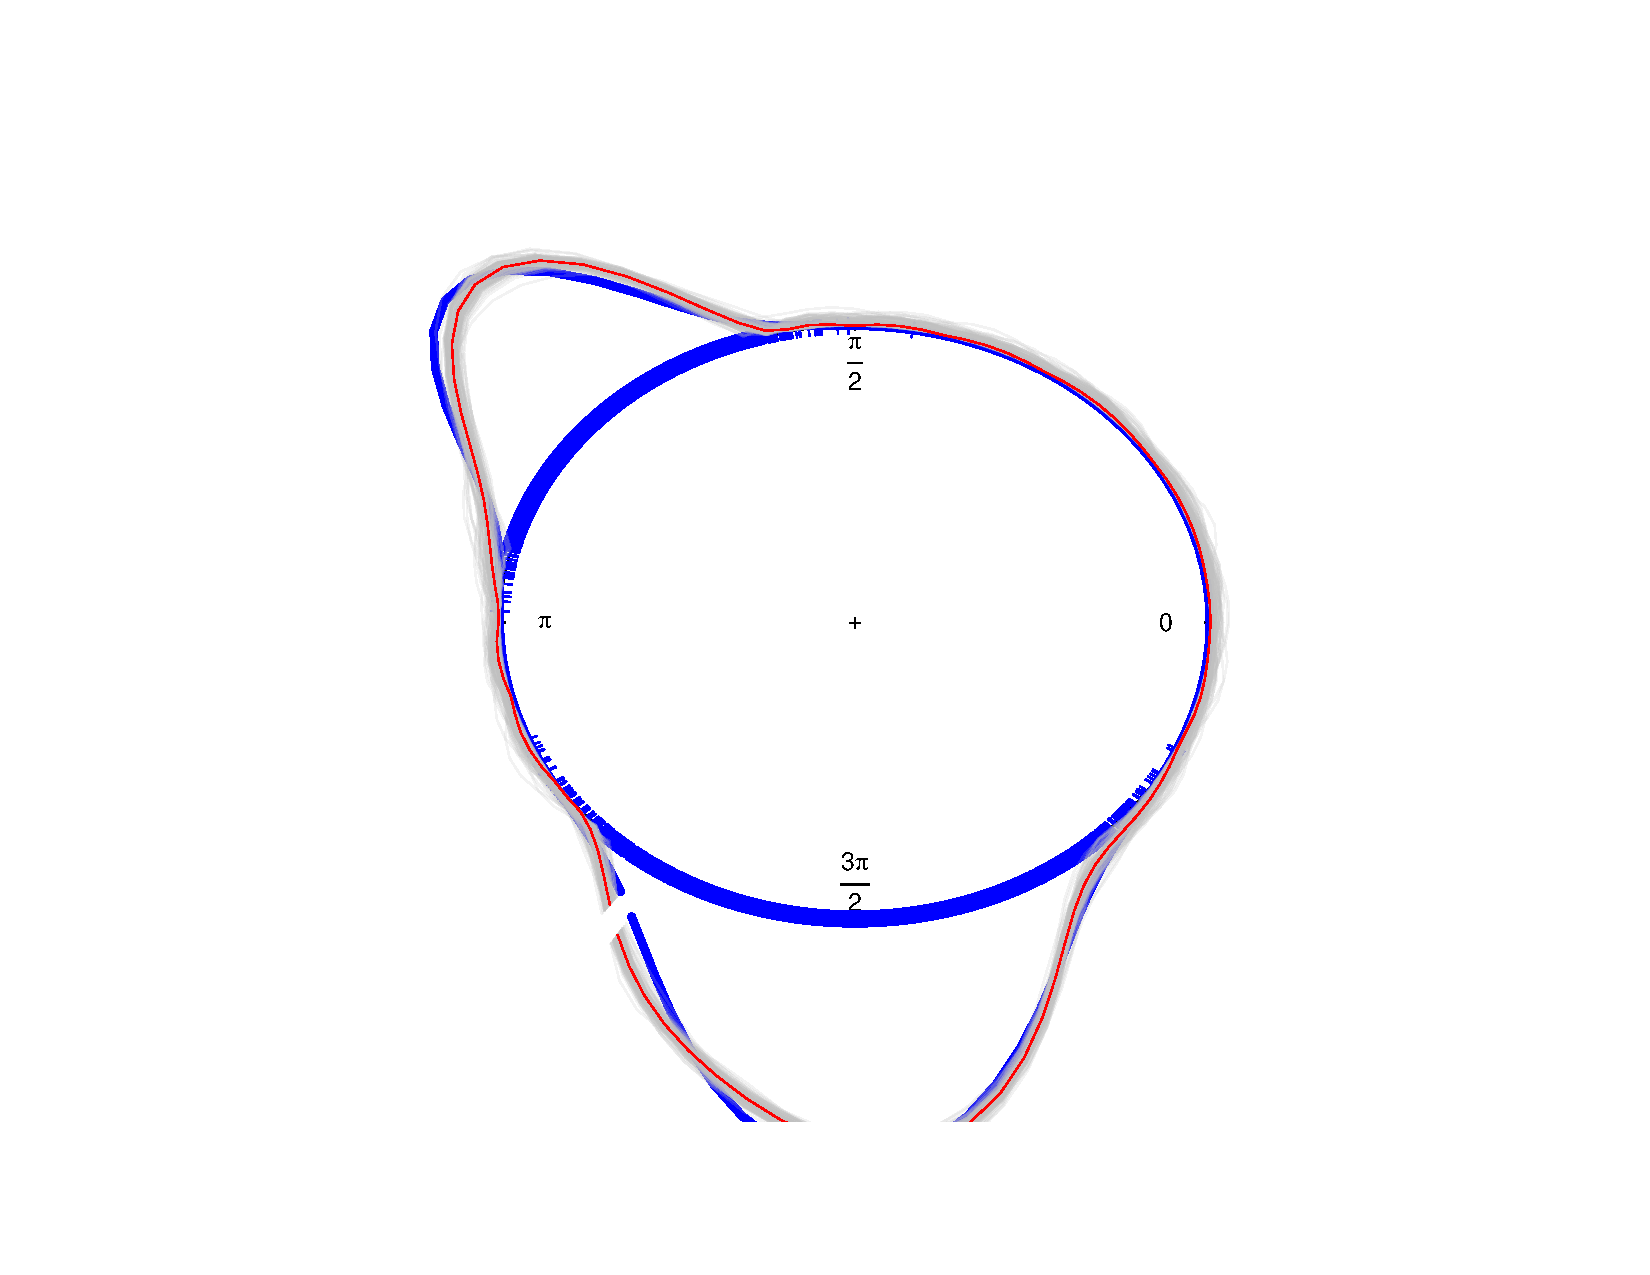
\includegraphics[width=.75\linewidth]{directsamp.pdf}
\caption{Sample from the posterior distribution and the posterior mean in the direct case}\label{M}
\end{figure}
\end{frame}
%
%\begin{frame}{Inverse problem : visualisation of the estimates}
%\begin{center}
%%	\animategraphics[loop,controls,width=40ex]{10}{compare/}{1}{91}
%\end{center}
%\end{frame}
%
%\begin{frame}{Inverse problem : empirical mean square errors of the estimates}
%\begin{figure}
%\centering
% 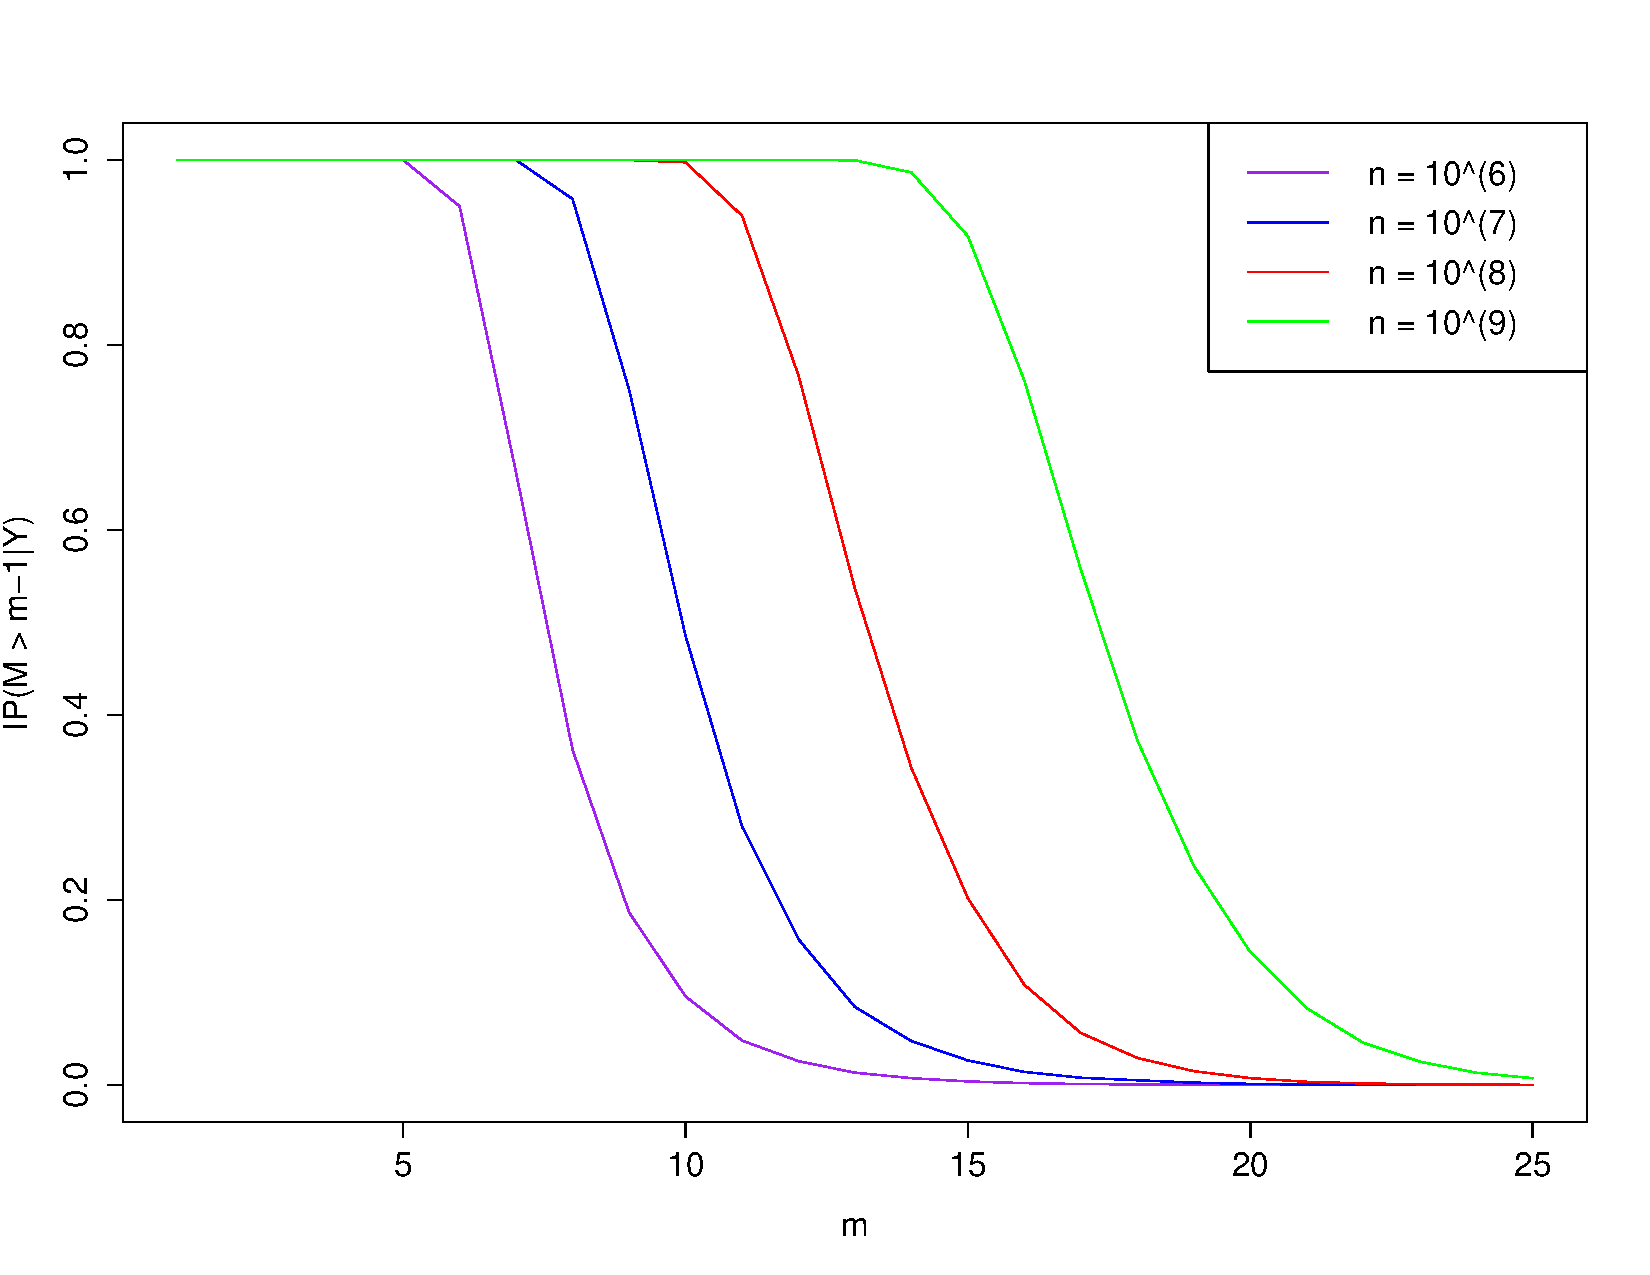
\includegraphics[width=.8\linewidth]{M.pdf}
%\caption{Evolution of the empirical mean squared error of the two estimates with respect to the number of observations in the direct case}\label{M}
%\end{figure}
%\end{frame}
%
%\begin{frame}{Inverse problem : sampling from the approximated posterior}
%\begin{figure}
%\centering
% 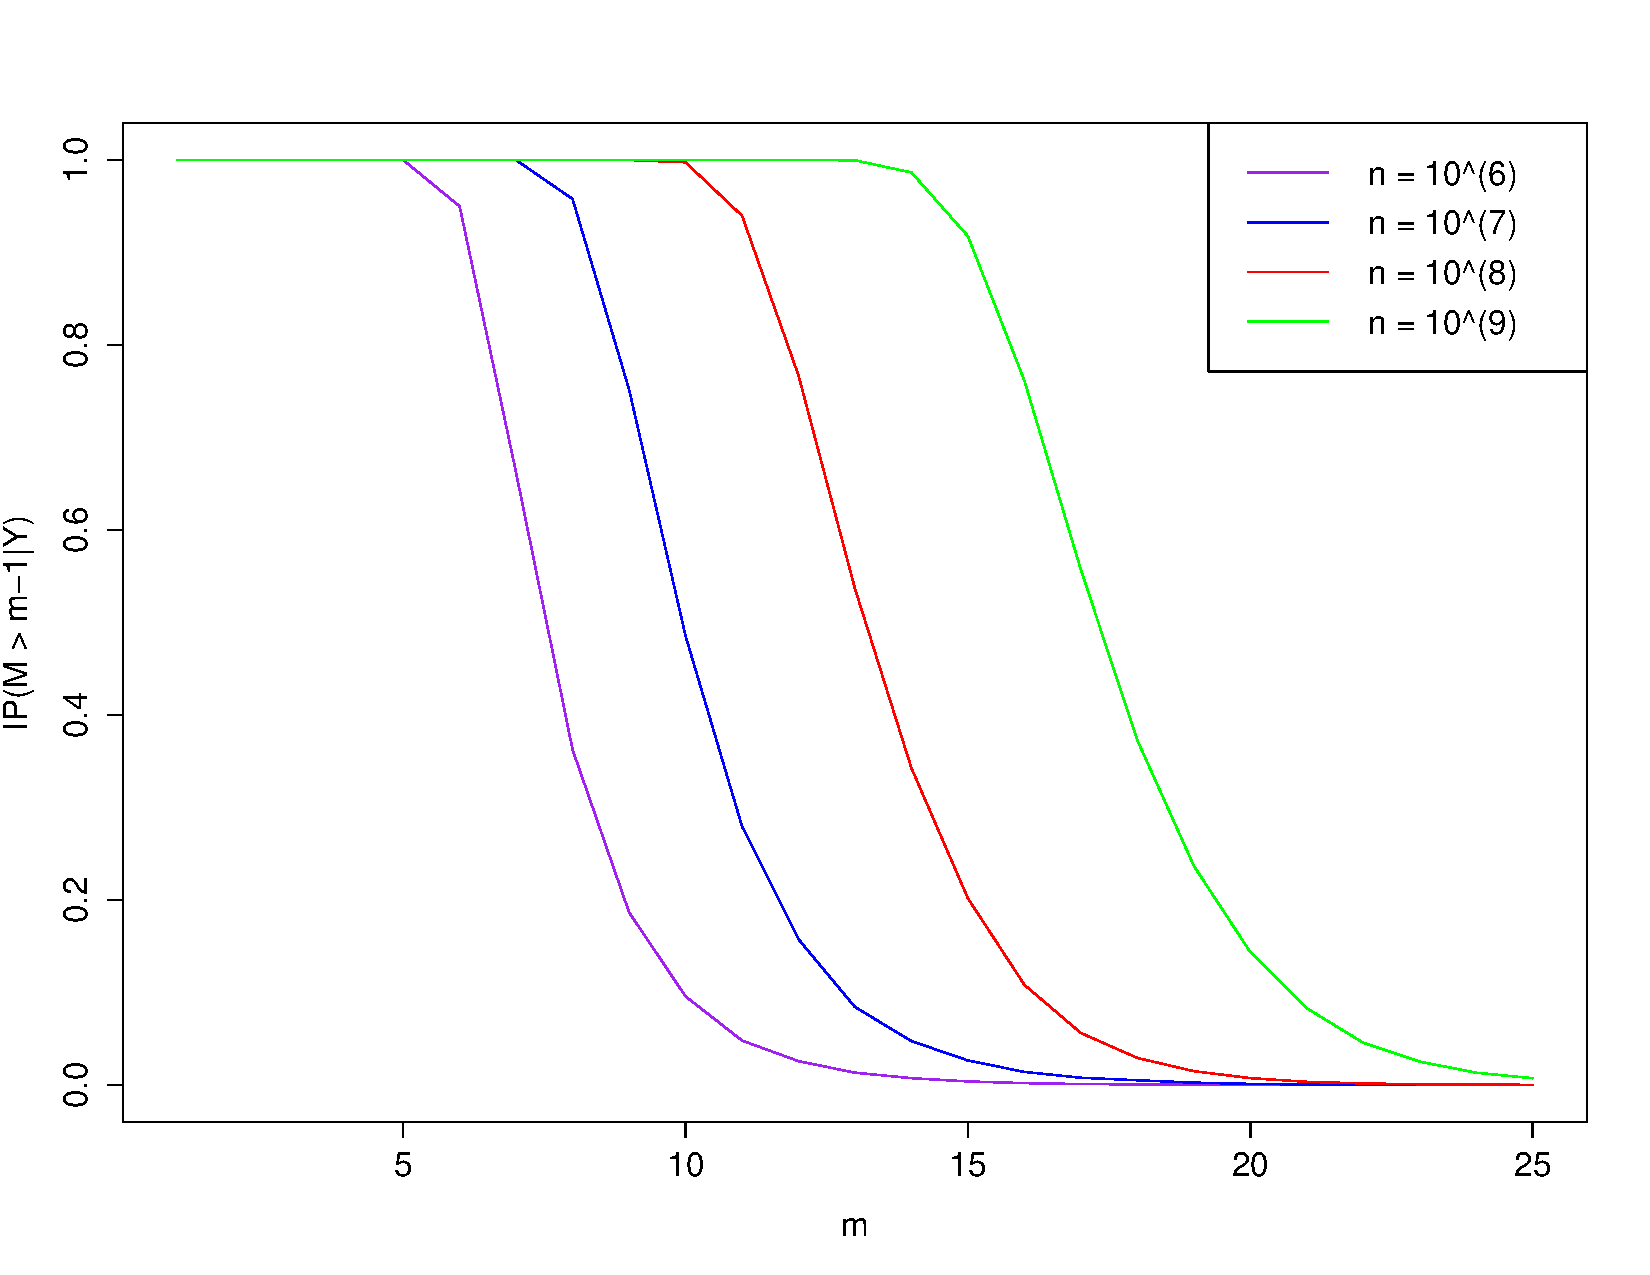
\includegraphics[width=.8\linewidth]{M.pdf}
%\caption{Sample from the posterior distribution and the posterior mean in the direct case}\label{M}
%\end{figure}
%\end{frame}

\begin{frame}{Summary}
\begin{itemize}
\item Bayesian method for circular deconvolution with interpretable prior ;
\item providing a fully data driven estimator, fulfilling oracle optimality ;
\item giving a Bayesian formulation of Oracle optimality...
\end{itemize}
And much more !
\begin{itemize}
\item Also fulfills minimax optimality (no $\log$ term !)
\item actually provides a complete family of optimal estimators using iterated posterior method
\item works with $\beta$-mixing dependance
\item suitable for severely ill-posed problems
\item can be adapted to real line deconvolution
\end{itemize}
\end{frame}

\begin{frame}<beamer:0>
\bibliography{iGSSM}
\end{frame}

\bibliographystyle{plainnat}
\end{document}